% Slide: Version Control System
\section{Version Control System}
\begin{frame}{Version Control System}
  \begin{itemize}
    \item What is a Version Control System?
    \begin{itemize}
      \item Manages changes in files (code/plain text).
      \item Creates versions/revisions.
      \item Reviews change history and traces changes.
      \item Restores previous versions.
    \end{itemize}
    \item Benefits:
    \begin{itemize}
      \item Useful for collaborative and individual work.
    \end{itemize}
    \item Tools:
    \begin{itemize}
      \item CVS (1986, deprecated).
      \item SVN (2000, centralized, heavy branches).
      \item Git (2005, distributed, light branches).
      \item Mercurial (2005, simpler but less flexible).
    \end{itemize}
  \end{itemize}
\end{frame}

% Slide: Git Overview
\section{Git Overview}
\begin{frame}{Git Overview}
  \begin{itemize}
    \item Created by Linus Torvalds in 2005 for Linux kernel development.
    \item Free, open source (GPL v2 license).
    \item Available for Linux, Windows, MacOS, BSD, Solaris.
    \item Features:
    \begin{itemize}
      \item Distributed collaboration.
      \item Supports multiple, concurrent lines of development.
    \end{itemize}
    \item Hosting platforms: Bitbucket, GitLab, GitHub.
    
\includegraphics[width=0.5\linewidth]{trainingmaterials/git-I/giticon.pdf}
  \end{itemize}
\end{frame}

% Slide: Git Basic Concepts

\begin{frame}{Git Basic Concepts}
  \begin{itemize}
    \item Repository:
    \begin{itemize}
      \item Container of the project files and versions.
      \item Contains the multiple versions of each file
    \end{itemize}
    \item Remote Repository:
    \begin{itemize}
      \item Located on a server, accessible by all developers.
    \end{itemize}
    \item Local Repository:
    \begin{itemize}
      \item Developers clone a copy of the remote repository (git clone)
      \item Changes are committed locally and pushed to the remote repository (git add and git commit)
      \item Changes are pushed to remote repos (git push)
      \item Changes are pulled from remote repos (git pull)
    \end{itemize}
  \end{itemize}
\end{frame}

\begin{frame}{Git Basic Concepts II}
    \centering
    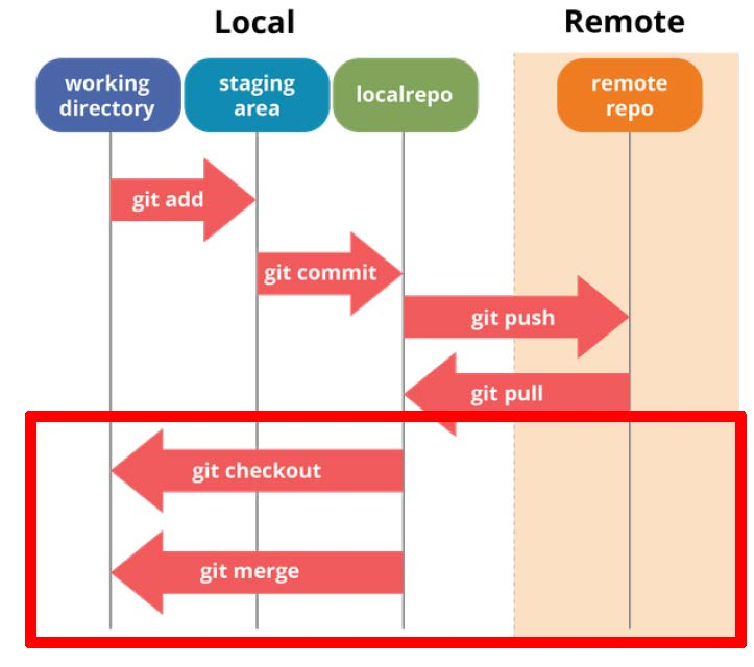
\includegraphics[width=0.5\linewidth]{trainingmaterials/git-I/gitflow.pdf }
\end{frame}
% Slide: Creating a Repository

\begin{frame}{Creating a Repository}
  \begin{enumerate}
    \item Create an account at \href{https://bitbucket.org}{Bitbucket.org} using your UPM email.
    \item Create a repository named \textit{NameInitialLastName\_ESD} (e.g., \textit{mruiz\_ESD}).
    \item Set project to \textbf{ESD}.
    \item Add instructors with read access:
    \begin{itemize}
      \item c.gonzalezb@alumnos.upm.es
      \item mariano.ruiz@upm.es
    \end{itemize}
  \end{enumerate}
\end{frame}

% Slide: Setting Up a Workspace

\begin{frame}{Setting Up a Workspace}
  \begin{enumerate}
    \item Install Git from \href{https://git-scm.com/downloads}{git-scm.com/downloads}. For example in Ubuntu: sudo apt install git
    \item Clone the repository:
    \begin{itemize}
      \item Command: \texttt{git clone <repository URL>}.
    \end{itemize}
    \item Create folders and files in the cloned repository.
    \item Commit changes:
    \begin{itemize}
      \item \texttt{git add <file\_path>}.
      \item \texttt{git commit}.
    \end{itemize}
    \item Push changes to the repository:
    \begin{itemize}
      \item \texttt{git push origin main}.
    \end{itemize}
  \end{enumerate}
\end{frame}

% Slide: Classwork/Homework
\section{Classwork/Homework}
\begin{frame}{Classwork/Homework}
  \begin{itemize}
    \item Create your repository and set up the environment (username, email).
    \item Invite instructors to your repository.
    \item Familiarize yourself with Git commands (commit, push, pull).
    \item Use the Bitbucket webpage to inspect changes.
    \item Clone the repository on another computer and test commits/pushes.
    \item Research:
    \begin{itemize}
      \item Updating a clone with changes from another clone.
      \item Using a \texttt{.gitignore} file.
      \item Understanding \texttt{origin} and \texttt{main}.
    \end{itemize}
  \end{itemize}
\end{frame}

